\documentclass[12pt]{unlsilabsop}
\title{Module assembly: Deliveries of BBM}
\date{May 6, 2019}
\author{Jose Andres Monroy}
\approved{Jose Andres Monroy}
\sopid{001}
\sopversion{v1}
\sopabstract{Describes the procedures to meassure the thermal resistance of the mock modules.}
\begin{document}

\maketitle

%------------------------------------------------------------------
\section{Scope}
This is regular procedure during the TFPX Phase II R\%D stage.

%------------------------------------------------------------------
\section{Purpose}
Determination of the thermal resistance is fundamental to characterize the cooling process; in particulater to model the thermal runaway (more details needed here).

%------------------------------------------------------------------
%>\section{Definitions}

%------------------------------------------------------------------
\section{Intro}
When the module is  
\begin{itemize}
    \item xxx
\end{itemize}

%------------------------------------------------------------------
\section{Equipment}

\begin{itemize}
    \item TDK-Lambda power supply.  
    \item Cables
    %\item Digital Multmeters (DVM)
    \item Bread board
    \item Mock module
    \item FLIR E50 IR camera (including tripod)
    \item Laptop
    \item 
\end{itemize}

%------------------------------------------------------------------
\section{Procedure}

\begin{enumerate}
    \item Mount the circuit according to the schematic in the Figure \ref{thermal_res_circuit}
      \begin{center}
        \begin{figure}[h]
          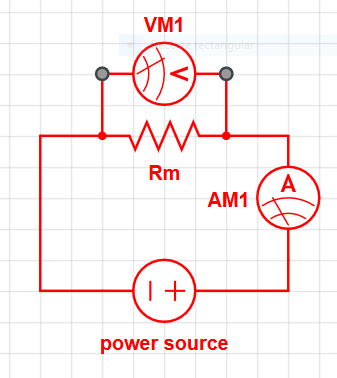
\includegraphics[width=0.5\textwidth]{img/Rm_circuit.png}
          \caption{Thermal resistance measurement circuit.}
          \label{setup}
        \end{figure}
      \end{center}

    \item Handle BBM only with proper protection: ESD wristband, gloves, face mask.
    \item Use vacuum pen of probe station for handling BBM. Don't use tweezers. If you have to flip a BBM, put it on a sheet of dust-free tissue and flip it carefully as demonstrated by your trainer. Touching a module with your hands should be avoided.
    \item Remove GelPak boxes from conductive plastic bag, use scissors to cut bag, if needed.
    \item Remove plastic clip and open GelPak boxes and get a first impression: Shipment should be complete, in order and no immediate damage is visible. Document if shipment deviates. Reject broken modules or modules with damaged/missing ROC.
    \item Compare list with delivery statement. Report any inconsistency in documentation and inform shipper.
    \item With the shipment confirmation email there comes an Excel spreadsheet. Open it in Excel and save a copy in ``Excel XML Spreadsheet 2003'' format. If shipment is incomplete, delete non-delivered lines prior saving in xml-format. Upload this xml-file using the ``Batch Module Submit'' functionality. Make sure to select ``Nebraska'' for the location and hit ``SUBMIT''. If successful, the newly received modules become listed in the part list. This step does the translation from the bump-bonding manufacturer's naming convention to the Purdue convention.

    Should the upload not work, do the upload manually using ``Module Submit''. If doing so, the translation of the manufacturer id to the Purdue convention has to be made manually, see SOP~000 for details. This needs to be done for every module.
    \item To document the following steps, retrieve the module via ``MAIN MENU''$\rightarrow$``Part List'', go to the BBM list (``Bare Module'') and click on the identifier you want to update. Click on the link ``Update Status'' to update any status.
    \item Place the GelPak on the special vacuum chuck and turn the vaccum on. Now you can pick a BBM with the vacuum pen with only minimal force when lifting off the GelPak.
    \item Perform the visual inspection of BBM according to SOP~202. Promote the status to ``Inspected'' for every module, leaving comments for findings and adding pictures as needed.
    \item Perform the IV test of BBM according to SOP~203. Upload data to database and promote status to ``IV Tested'' for every module tested.
    \item Failed BBM should be clearly marked on the outside of the box. Shipper needs to be informed and action taken.
    \item Document any other findings not mentioned already in the database.
    \item Close and secure the GelPak with the clip. Place it in the dry-air storage cabinet on a tray foreseen for BBM.
\end{enumerate}
Deliveries on dicing tape instead of GelPak boxes are not acceptable any more and need to be rejected. Removal of BBM from dicing tape is a delicate procedure and should only be performed if trained properly.

The person performing the steps above may choose to perform the visual inspection and the IV test in sequence or in parallel.

%------------------------------------------------------------------
\section{Documentation}
Everything needs to be documented in the Purdue database per the instructions above. If nothing special is to report, no documentation is needed in the UNL elog.

\end{document}

